\documentclass[11pt, a4paper]{article}
\usepackage[utf8]{inputenc}
\usepackage{geometry}
\usepackage{graphicx}
\usepackage[dvipsnames]{xcolor}
\geometry{margin=1in}
\setlength{\parindent}{0em}
\setlength{\parskip}{1em}
\title{Computação gráfica | Trabalho 1}
\author{Professor: Waldemar Celles\\
Aluno: Antenor Barros Leal}
\date{29 de setembro de 2024}
\begin{document}
\maketitle

\section {Resumo}
Este trabalho tem como objetivo de fazer uma representação parcial do sistema solar.
São mostrados o sol, mercúrio e a Terra com a Lua.

\section {Escalas}

As escalas e distância dos planetas em relação ao sol não são realistas, já que, para
isto seria difícil ver os planetas, eles teriam que ficar muito pequenos. Porém as
relações entre os períodos de órbita são realistas.

Observando a classe da engine vemos um valor padrão de 365. Este é o período de órbita.

Tem-se que multiplicar por 1000 para que o movimento fique perceptível e também multiplicar 
por t-t0 para que o movimento seja agnóstico em relação a velocidade do computador.
T-T0 é o momento que a função de atualização foi chamada menos o momento da chamada
anterior. Ou seja, o período de chamada de update().

\section{Diagrama}

Observe o diagrama de clases abaixo.

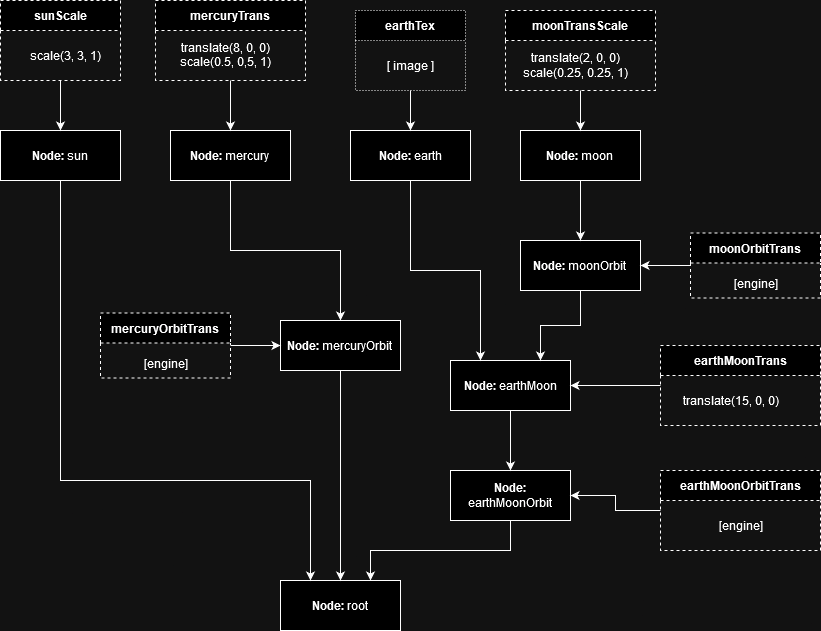
\includegraphics[width=0.8\linewidth]{Trab1Graph.png}

Para que a imagem de fundo fique por trás de todos os astros foi usada a componente z
do scale. Note que a transformação "spaceTrans" possui zero na componente z do translate,
as transformações para os outros astros usando um na componente z. 

\end{document}